\documentclass[xcolor=dvipsnames]{beamer}
\mode<presentation>

\setbeamertemplate{itemize item}[ball]
%\usetheme[secheader]{Boadilla}
%\usetheme{boxes}
\usetheme{myBoadilla}
%\usetheme[secheader]{myBoadilla}
%\usetheme[left]{Goettingen}

%\usepackage{CSIC2}
\setbeamertemplate{itemize item}[ball]
 \setbeamertemplate{navigation symbols}{
      \insertslidenavigationsymbol
%%      \insertdocnavigationsymbol 
%%    {\footnotesize \insertframenumber} %% FIXME: delete if we use CSIC2
 }

\usepackage[absolute,overlay]{textpos}
\usepackage[english]{babel}
\usepackage[latin1]{inputenc}
\usepackage{times}
\usepackage[T1]{fontenc}
% Or whatever. Note that the encoding and the font should match. If T1
% does not look nice, try deleting the line with the fontenc.
%%\usepackage{fancybox}
\usepackage[lined]{algorithm2e}

\usepackage{url}
\newcommand{\cyan}[1]{{\textcolor {cyan} {#1}}}
\newcommand{\blu}[1]{{\textcolor {blue} {#1}}}
\newcommand{\Burl}[1]{\blu{\url{#1}}}
\newcommand{\red}[1]{{\textcolor {red} {#1}}}
\newcommand{\green}[1]{{\textcolor {green} {#1}}}
\newcommand{\mg}[1]{{\textcolor {magenta} {#1}}}
\newcommand{\og}[1]{{\textcolor {PineGreen} {#1}}}
\newcommand{\code}[1]{\texttt{\slshape\footnotesize #1}}
\newcommand{\myverb}[1]{{\footnotesize\texttt {\textbf{#1}}}}
\newcommand{\Rnl}{\ +\qquad\ }
\newcommand{\Emph}[1]{\emph{\mg{#1}}}
\newcommand{\gry}[1]{{\textcolor {gray} {#1}}}

\newcommand{\hanging}[1]{ 
\renewcommand{\baselinestretch}{0.7}\small\normalsize
\setlength{\parskip}{1.5ex plus0ex minus0ex}
  \noindent\hangindent=24pt
  \hangafter=1 
   {\scriptsize #1}
  %\hangindent\parindent
}   


\newcommand{\hango}[1]{ 
\renewcommand{\baselinestretch}{0.7}\small\normalsize
\setlength{\parskip}{1.5ex plus0ex minus0ex}
  \noindent\hangindent=24pt
  \hangafter=1 
   {\tiny #1}
  %\hangindent\parindent
}   


\newcommand{\hanginp}[2]{ 
  \renewcommand{\baselinestretch}{0.7}\small\normalsize
  \setlength{\parskip}{1.5ex plus0ex minus0ex}
  \noindent\hangindent=24pt
  \hangafter=1 
  {\scriptsize #1}{\hspace{2pt}\Large\red{#2}}
  % \hangindent\parindent
}   


%% use for itemize wihtin description
% \newenvironment{myitemize} {
%   \setlength{\leftmarginii}{-10mm}
%   \itemize
% }

% \newenvironment{myitemize}
% {\setlength{\leftmarginii}{-10mm}
% \begin{itemize}}
% {\end{itemize}}


\newenvironment{myitemize}
{\begin{itemize}}{\end{itemize}}


\newcommand{\mydes}[2][]{
  \vspace*{-1pt}
%%  \renewcommand{\baselinestretch}{0.7}\small\normalsize
  \begin{description}\item[{#2}]{#1}\end{description}
\vspace*{-8pt}
}


\usepackage{gitinfo}


\title{BM-1: a 10 minute intro}
\subtitle{Critical analysis of scientific
literature. Applied statistics for molecular biosciences (BM-1)}



\author[R. Diaz-Uriarte]{Ram�n Diaz-Uriarte} %% \\ \Burl{http://ligarto.org/rdiaz}}

\institute[]{Department of Biochemistry\\
Universidad Aut�noma de Madrid\\
Madrid, Spain\\
\texttt{ramon.diaz@iib.uam.es}\\
\Burl{http://ligarto.org/rdiaz}
}


% \date[22-09-2014]{22-September-2014}
% \date{\gitAuthorDate\ {\footnotesize (Rev: \gitAbbrevHash)}}
\date[12-09-2016]{12-September-2016\\ {\tiny (Rev: \gitAbbrevHash)}}


\begin{document}


\begin{frame}
  \titlepage
\end{frame}


% \begin{frame}
%    \frametitle{Outline}
%  {\small
%  \tableofcontents[subsectionstyle=hide]
%  }
%  \end{frame}



% \begin{frame}
%   \frametitle{Organization and long presentation of BM-1}
%   \begin{itemize}
%   \item Monday, 22-September-2014, 10:00 (am, of course!), Aula Magna
%   \end{itemize}
% \end{frame}



\begin{frame}
  \frametitle{Your homework for tomorrow}
  \begin{itemize}
  \item Make sure you can access Moodle:
    \Burl{http://moodle.uam.es}
  %% \item Course URL: \Burl{https://moodle.uam.es/course/view.php?id=22524}
  \end{itemize}
\end{frame}



% \begin{frame}
%   \frametitle{What Moodle will look like}
% \vspace*{10pt}
%    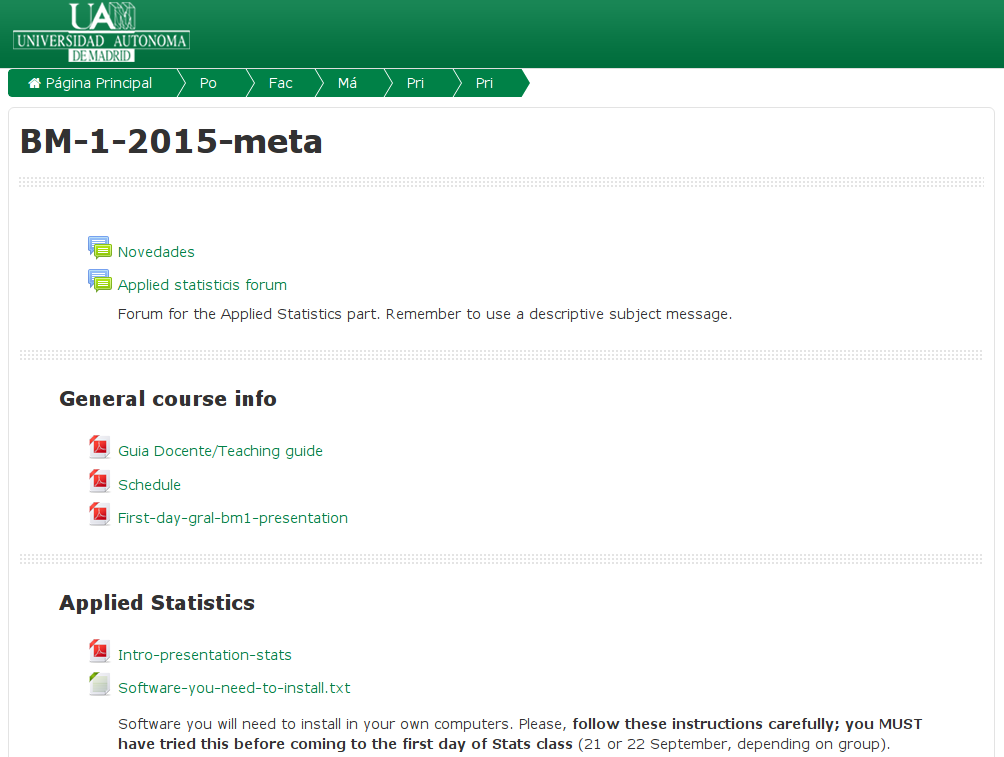
\includegraphics[%
%    width=12.5cm,
%    keepaspectratio]{moodle-view.png}
% \end{frame}





% \begin{frame}
%   \frametitle{Your homework for tomorrow}
%   \begin{itemize}
%   %% \item You should have received an email about BM-1.
%   \item If problems with Moodle, come tomorrow Tuesday 15 September to
%     Seminarios 4 and 5, from 10:00 to 12:00 (better if you are there at
%     10:00).
%   \end{itemize}
% \end{frame}




\begin{frame}
  \frametitle{What Moodle is this? Why do I need it?}
  \begin{itemize}
  \item This is the usual UAM moodle.
  \item \red{We will use it for exams.}
  \item We will use it to upload course material, self-evaluation
    exercises, etc.
  \end{itemize}
\end{frame}


% \begin{frame}
%   \frametitle{How Moodle looks like}
%   {\tiny (Something similar to this ---details might vary. 
%     This presentation is  ``First-day-gral-bm1-presentation'')}

% \vspace*{10pt}


%    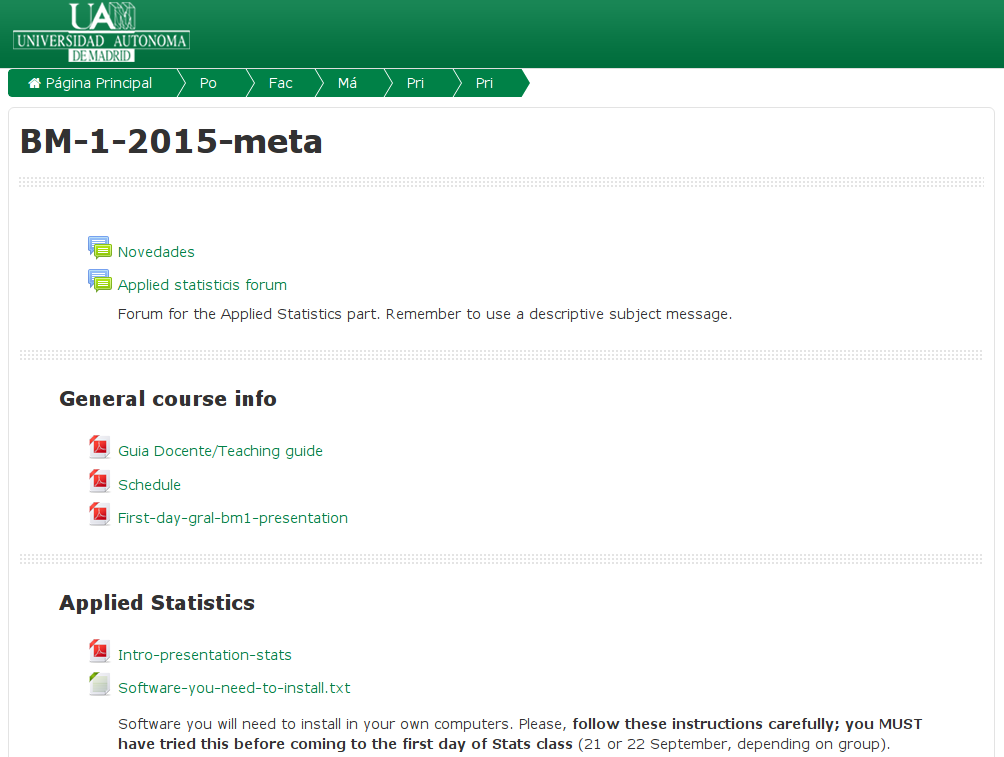
\includegraphics[%
%    width=11.5cm,
%    keepaspectratio]{moodle-view.png}
% \end{frame}



\begin{frame}
  \frametitle{Other homework (ASAP)}
  \begin{enumerate}
  \item Get your UAM email: all issues to CAU (google for ``UAM cau
    email''). No UAM email, no Moodle.
  \item {\scriptsize (If you plan on using your computer around campus)} Enable Wifi
    access (google for ``UAM wifi'').
  \end{enumerate}
\end{frame}


% \begin{frame}
%   \frametitle{Software for BM-1}
%   \begin{itemize}
%   \item An updated list available by 19-September (Moodle, of course).
%   \end{itemize}
% \end{frame}



\begin{frame}
  \frametitle{Schedule}
  \begin{itemize}
  \item Available from Moodle (file ``Schedule'').

  \item There are two groups (A and B). You will  be told which
    group you belong to.
  \item For scientific communication, there are subgroups (more details
    later).
  \item Pay attention to Schedule! % E.g., Applied statistics, 24, 25, and
  %   28 September, for groups A and B.
  % \item Seminars for team work in Schedule too.
  \end{itemize}
\end{frame}



% \begin{frame}
%   \frametitle{How the schedule looks like}
% \vspace*{10pt}
%    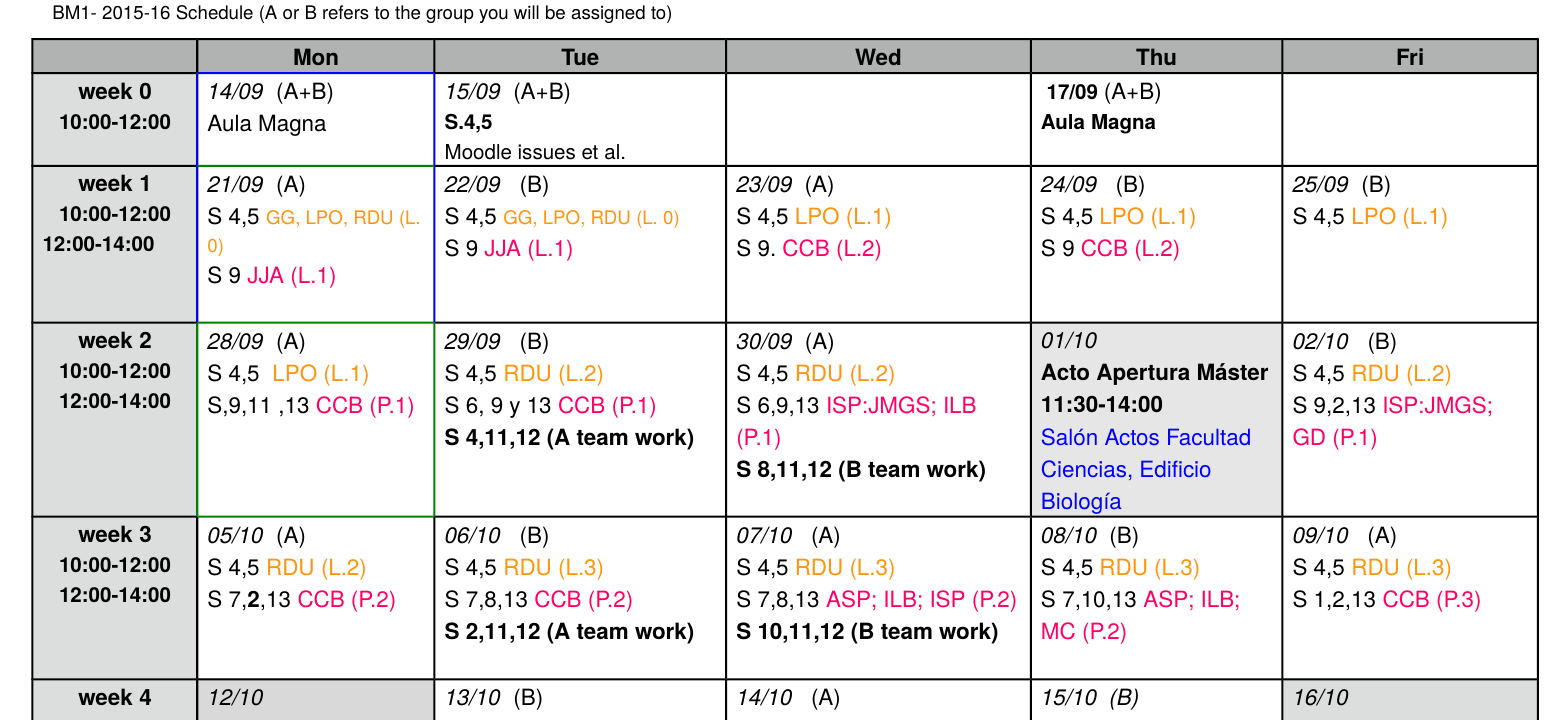
\includegraphics[%
%    width=12.5cm,
%    keepaspectratio]{schedule-view.png}
% \end{frame}



% \begin{frame}
%   \frametitle{Schedule: key dates}
% Key dates until 21-September:
%     \begin{description}
%     \item[Access to Moodle] 15-September, Seminarios 4 y 5. 10:00--12:00.
%     \item[Aula Magna talk] 17-September. Aula Magna. 10:00--12:00.
% %%    \item[I.\ Fari�as' talk] 19-September. Aula Magna. 10:00--12:00.
%     \item[First class BM-1] 21 and 22-September (groups A and B, respectively)
%       \begin{itemize}
%       \item Seminars 4 and 5 (stats). 10:00--12:00.
%       \item Seminar 9 (scientific communication). 12:00--14:00. 
%       \end{itemize}
%     \end{description}
%     \vspace*{15pt} 

% {\footnotesize (Did we say all are mandatory, except
%       tomorrow's Moodle session ---if you got it working?)}

% \vspace*{15pt}
% Remember also \textbf{Acto Apertura M�ster}, 1-October, Facultad Ciencias,
% Sal�n Actos, Edificio Biolog�a.
% \end{frame}



\begin{frame}
  \frametitle{Warning!}

  This is a preliminary version of this document and can suffer changes
  before 12-09-2016.
  % \begin{itemize}
  % \item
  % \item
  % \end{itemize}
\end{frame}


% \begin{frame}
%   \frametitle{A copy of this PDF?}
% \Burl{http://ligarto.org/rdiaz/First-day-BM1.pdf}
% \end{frame}


\end{document}


%%% Local Variables:
%%% mode: latex
%%% TeX-master: t
%%% End:







